% Hosting placement study (direction 4). Standalone subsection: % Hosting placement study (direction 4). Standalone subsection: % Hosting placement study (direction 4). Standalone subsection: % Hosting placement study (direction 4). Standalone subsection: \input{placement_section}
% from main.tex where it fits (Experiments and Analysis). Numbers: results/placement_summary.md.
\subsection{Hosting the two halves on different devices}
\label{sec:placement}

A flow-matching VLA step has two halves joined by one handoff: the prefix (vision tower and
VLM, run once, filling the KV cache) and the action-expert loop (ten flow steps over that
cache). We host each half on its own device and time the parts and the whole step for five
placements: both halves on one GPU, prefix and loop on two GPUs, loop on the host CPU, prefix
on the host CPU, and CPU only (Figure~\ref{fig:placement}). GPUs run FP16 and the CPU FP32.
The runs are on cuda2 (RTX 2080 Ti, Xeon E5-2660 v3, 20 threads pinned to the GPU's NUMA node);
the end-to-end step re-timed after all placements moved by 0.8\%.

\begin{figure}[t]
  \centering
  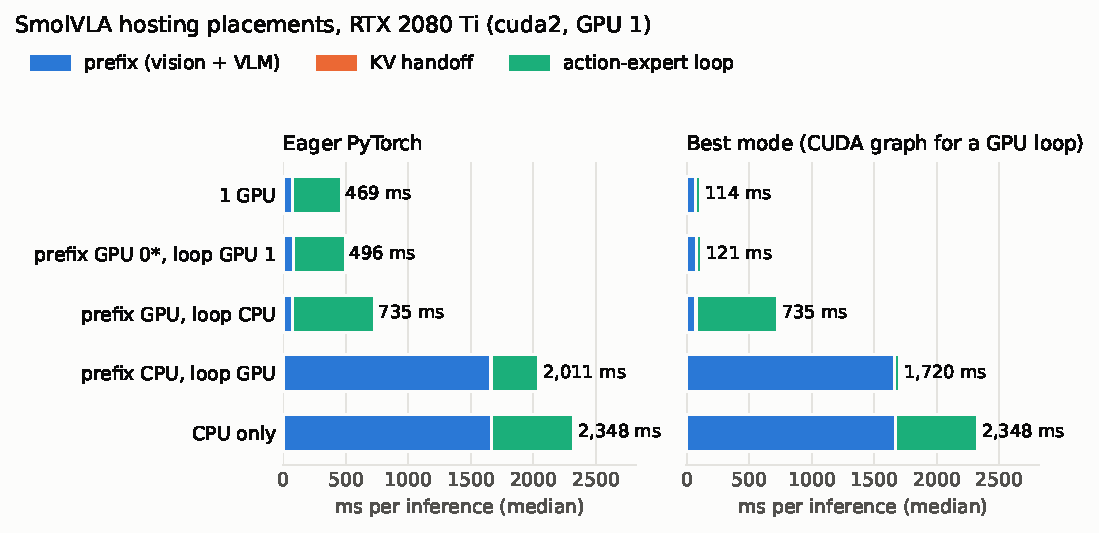
\includegraphics[width=\linewidth]{figures/placement_cuda2.pdf}
  \caption{SmolVLA step time per placement on cuda2, split into prefix, KV handoff (1.5 to
  3.2\,ms, too small to see) and action-expert loop. Left: eager PyTorch. Right: CUDA graph for
  the loop when it runs on a GPU. All rows use the healthy GPU~1, except the two-GPU row, whose
  prefix ran on GPU~0 while that GPU was stuck at a reduced clock (*, about 5\,ms slower).}
  \label{fig:placement}
\end{figure}

\paragraph{The handoff is cheap and the step is additive.} The KV cache is 4.9\,MB in 33
tensors. Moving it costs 1.5\,ms GPU to GPU, 2.8\,ms GPU to CPU and 3.2\,ms CPU to GPU (FP32
cache cast on the GPU), 1 to 3\% of the best single-GPU step (114\,ms). The parts timed alone
sum to the end-to-end step within 1.6\% in every placement, so a split placement can be
predicted from single-device runs:
$T(A,B) = T_\mathrm{prefix}(A) + n\,t_0 + S/\mathit{BW}_{A\to B} + T_\mathrm{loop}(B)$, with
$t_0$ and $\mathit{BW}$ from a copy calibration and each device's own baseline. The prediction
is within 0.1\% for the GPU-CPU split, 2.3\% (eager) and 0.6\% (graph loop) for the CPU-GPU
split, and 0.2\% (graph loop) and 2.5\% (eager) for the two-GPU split. Splitting does not
shorten one inference, since the halves run in sequence; it adds capacity, which hosting
several policies on one GPU (Section~\ref{sec:multipolicy}) provides more cheaply.

\paragraph{The CPU is not a useful host.} The prefix is 23 times slower on the CPU than on the
GPU, and CPU-only inference is 21 times slower than the best single-GPU step. The action loop
on 20 CPU threads takes 650\,ms, only 1.7 times the eager GPU loop (389\,ms): eager PyTorch is
so dispatch bound that a CPU comes close to it. With a CUDA graph the GPU loop takes 40\,ms, 16
times faster than the CPU. On the TITAN V host (24 threads) the CPU loop is 3.3 times the eager
loop and 14 times the graph loop.

\paragraph{Graph mode exposes a faulty GPU.} During these experiments GPU~0 of cuda2 ran the
graph loop in 54.1\,ms against 39.6\,ms on GPU~1, while the eager step was 482\,ms on both:
host-bound eager execution hides the difference and graph mode exposes it. GPU~0 is not slower
by design. A week earlier it held 1,950\,MHz under load and ran a C++ replay of the loop as
fast as GPU~1; since then it idles stuck in the P0 power state at 1,350\,MHz with no clock
event reason, and $1950/1350 = 1.44$ is close to the $1.37$ loop ratio. As with the TITAN V
(Section~\ref{sec:crossgpu}), the clock a GPU actually runs at sets the graph-mode latency.
Our runner now records every GPU's power state and clock and refuses a GPU that idles in P0.
% Needs \label{sec:crossgpu} on main.tex's "Cross-GPU accuracy" subsection (sustained-clock
% finding) and \label{sec:multipolicy} on the multi-policy subsection (branch
% shrikar/multipolicy-hosting); drop that clause if it is not in the paper.

% from main.tex where it fits (Experiments and Analysis). Numbers: results/placement_summary.md.
\subsection{Hosting the two halves on different devices}
\label{sec:placement}

A flow-matching VLA step has two halves joined by one handoff: the prefix (vision tower and
VLM, run once, filling the KV cache) and the action-expert loop (ten flow steps over that
cache). We host each half on its own device and time the parts and the whole step for five
placements: both halves on one GPU, prefix and loop on two GPUs, loop on the host CPU, prefix
on the host CPU, and CPU only (Figure~\ref{fig:placement}). GPUs run FP16 and the CPU FP32.
The runs are on cuda2 (RTX 2080 Ti, Xeon E5-2660 v3, 20 threads pinned to the GPU's NUMA node);
the end-to-end step re-timed after all placements moved by 0.8\%.

\begin{figure}[t]
  \centering
  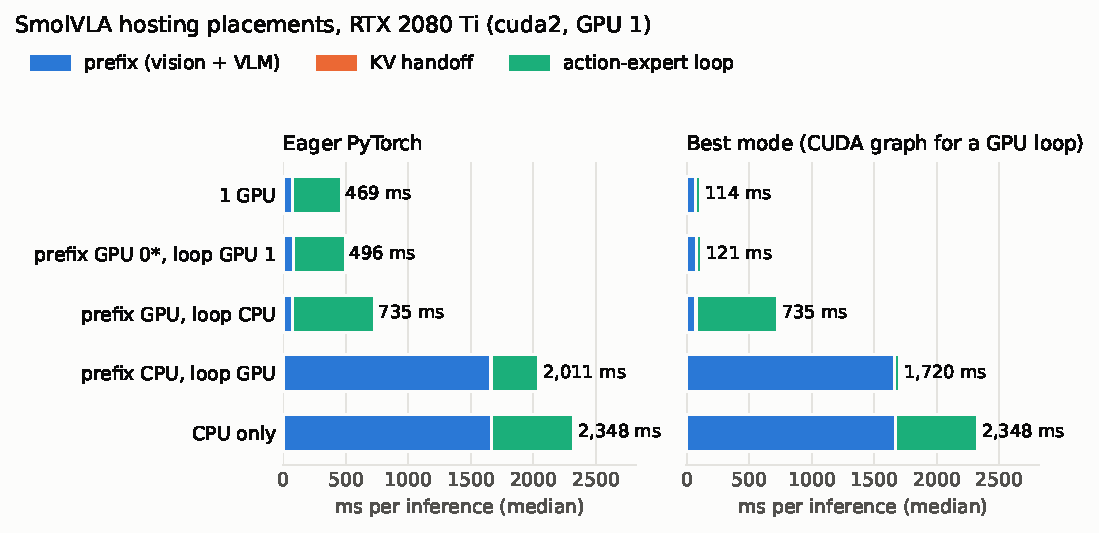
\includegraphics[width=\linewidth]{figures/placement_cuda2.pdf}
  \caption{SmolVLA step time per placement on cuda2, split into prefix, KV handoff (1.5 to
  3.2\,ms, too small to see) and action-expert loop. Left: eager PyTorch. Right: CUDA graph for
  the loop when it runs on a GPU. All rows use the healthy GPU~1, except the two-GPU row, whose
  prefix ran on GPU~0 while that GPU was stuck at a reduced clock (*, about 5\,ms slower).}
  \label{fig:placement}
\end{figure}

\paragraph{The handoff is cheap and the step is additive.} The KV cache is 4.9\,MB in 33
tensors. Moving it costs 1.5\,ms GPU to GPU, 2.8\,ms GPU to CPU and 3.2\,ms CPU to GPU (FP32
cache cast on the GPU), 1 to 3\% of the best single-GPU step (114\,ms). The parts timed alone
sum to the end-to-end step within 1.6\% in every placement, so a split placement can be
predicted from single-device runs:
$T(A,B) = T_\mathrm{prefix}(A) + n\,t_0 + S/\mathit{BW}_{A\to B} + T_\mathrm{loop}(B)$, with
$t_0$ and $\mathit{BW}$ from a copy calibration and each device's own baseline. The prediction
is within 0.1\% for the GPU-CPU split, 2.3\% (eager) and 0.6\% (graph loop) for the CPU-GPU
split, and 0.2\% (graph loop) and 2.5\% (eager) for the two-GPU split. Splitting does not
shorten one inference, since the halves run in sequence; it adds capacity, which hosting
several policies on one GPU (Section~\ref{sec:multipolicy}) provides more cheaply.

\paragraph{The CPU is not a useful host.} The prefix is 23 times slower on the CPU than on the
GPU, and CPU-only inference is 21 times slower than the best single-GPU step. The action loop
on 20 CPU threads takes 650\,ms, only 1.7 times the eager GPU loop (389\,ms): eager PyTorch is
so dispatch bound that a CPU comes close to it. With a CUDA graph the GPU loop takes 40\,ms, 16
times faster than the CPU. On the TITAN V host (24 threads) the CPU loop is 3.3 times the eager
loop and 14 times the graph loop.

\paragraph{Graph mode exposes a faulty GPU.} During these experiments GPU~0 of cuda2 ran the
graph loop in 54.1\,ms against 39.6\,ms on GPU~1, while the eager step was 482\,ms on both:
host-bound eager execution hides the difference and graph mode exposes it. GPU~0 is not slower
by design. A week earlier it held 1,950\,MHz under load and ran a C++ replay of the loop as
fast as GPU~1; since then it idles stuck in the P0 power state at 1,350\,MHz with no clock
event reason, and $1950/1350 = 1.44$ is close to the $1.37$ loop ratio. As with the TITAN V
(Section~\ref{sec:crossgpu}), the clock a GPU actually runs at sets the graph-mode latency.
Our runner now records every GPU's power state and clock and refuses a GPU that idles in P0.
% Needs \label{sec:crossgpu} on main.tex's "Cross-GPU accuracy" subsection (sustained-clock
% finding) and \label{sec:multipolicy} on the multi-policy subsection (branch
% shrikar/multipolicy-hosting); drop that clause if it is not in the paper.

% from main.tex where it fits (Experiments and Analysis). Numbers: results/placement_summary.md.
\subsection{Hosting the two halves on different devices}
\label{sec:placement}

A flow-matching VLA step has two halves joined by one handoff: the prefix (vision tower and
VLM, run once, filling the KV cache) and the action-expert loop (ten flow steps over that
cache). We host each half on its own device and time the parts and the whole step for five
placements: both halves on one GPU, prefix and loop on two GPUs, loop on the host CPU, prefix
on the host CPU, and CPU only (Figure~\ref{fig:placement}). GPUs run FP16 and the CPU FP32.
The runs are on cuda2 (RTX 2080 Ti, Xeon E5-2660 v3, 20 threads pinned to the GPU's NUMA node);
the end-to-end step re-timed after all placements moved by 0.8\%.

\begin{figure}[t]
  \centering
  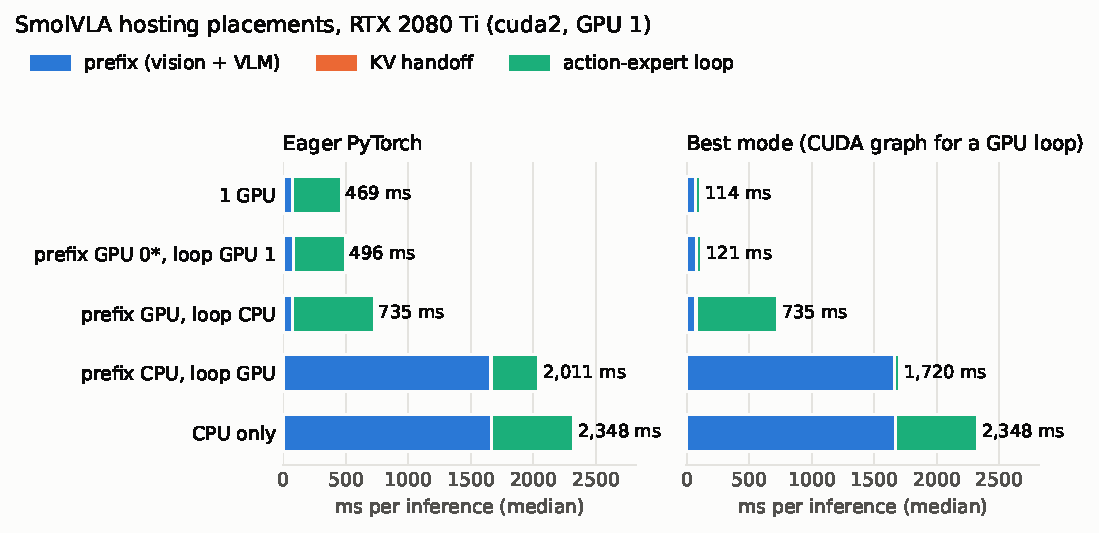
\includegraphics[width=\linewidth]{figures/placement_cuda2.pdf}
  \caption{SmolVLA step time per placement on cuda2, split into prefix, KV handoff (1.5 to
  3.2\,ms, too small to see) and action-expert loop. Left: eager PyTorch. Right: CUDA graph for
  the loop when it runs on a GPU. All rows use the healthy GPU~1, except the two-GPU row, whose
  prefix ran on GPU~0 while that GPU was stuck at a reduced clock (*, about 5\,ms slower).}
  \label{fig:placement}
\end{figure}

\paragraph{The handoff is cheap and the step is additive.} The KV cache is 4.9\,MB in 33
tensors. Moving it costs 1.5\,ms GPU to GPU, 2.8\,ms GPU to CPU and 3.2\,ms CPU to GPU (FP32
cache cast on the GPU), 1 to 3\% of the best single-GPU step (114\,ms). The parts timed alone
sum to the end-to-end step within 1.6\% in every placement, so a split placement can be
predicted from single-device runs:
$T(A,B) = T_\mathrm{prefix}(A) + n\,t_0 + S/\mathit{BW}_{A\to B} + T_\mathrm{loop}(B)$, with
$t_0$ and $\mathit{BW}$ from a copy calibration and each device's own baseline. The prediction
is within 0.1\% for the GPU-CPU split, 2.3\% (eager) and 0.6\% (graph loop) for the CPU-GPU
split, and 0.2\% (graph loop) and 2.5\% (eager) for the two-GPU split. Splitting does not
shorten one inference, since the halves run in sequence; it adds capacity, which hosting
several policies on one GPU (Section~\ref{sec:multipolicy}) provides more cheaply.

\paragraph{The CPU is not a useful host.} The prefix is 23 times slower on the CPU than on the
GPU, and CPU-only inference is 21 times slower than the best single-GPU step. The action loop
on 20 CPU threads takes 650\,ms, only 1.7 times the eager GPU loop (389\,ms): eager PyTorch is
so dispatch bound that a CPU comes close to it. With a CUDA graph the GPU loop takes 40\,ms, 16
times faster than the CPU. On the TITAN V host (24 threads) the CPU loop is 3.3 times the eager
loop and 14 times the graph loop.

\paragraph{Graph mode exposes a faulty GPU.} During these experiments GPU~0 of cuda2 ran the
graph loop in 54.1\,ms against 39.6\,ms on GPU~1, while the eager step was 482\,ms on both:
host-bound eager execution hides the difference and graph mode exposes it. GPU~0 is not slower
by design. A week earlier it held 1,950\,MHz under load and ran a C++ replay of the loop as
fast as GPU~1; since then it idles stuck in the P0 power state at 1,350\,MHz with no clock
event reason, and $1950/1350 = 1.44$ is close to the $1.37$ loop ratio. As with the TITAN V
(Section~\ref{sec:crossgpu}), the clock a GPU actually runs at sets the graph-mode latency.
Our runner now records every GPU's power state and clock and refuses a GPU that idles in P0.
% Needs \label{sec:crossgpu} on main.tex's "Cross-GPU accuracy" subsection (sustained-clock
% finding) and \label{sec:multipolicy} on the multi-policy subsection (branch
% shrikar/multipolicy-hosting); drop that clause if it is not in the paper.

% from main.tex where it fits (Experiments and Analysis). Numbers: results/placement_summary.md.
\subsection{Hosting the two halves on different devices}
\label{sec:placement}

A flow-matching VLA step has two halves joined by one handoff: the prefix (vision tower and
VLM, run once, filling the KV cache) and the action-expert loop (ten flow steps over that
cache). We host each half on its own device and time the parts and the whole step for five
placements: both halves on one GPU, prefix and loop on two GPUs, loop on the host CPU, prefix
on the host CPU, and CPU only (Figure~\ref{fig:placement}). GPUs run FP16 and the CPU FP32.
The runs are on cuda2 (RTX 2080 Ti, Xeon E5-2660 v3, 20 threads pinned to the GPU's NUMA node);
the end-to-end step re-timed after all placements moved by 0.8\%.

\begin{figure}[t]
  \centering
  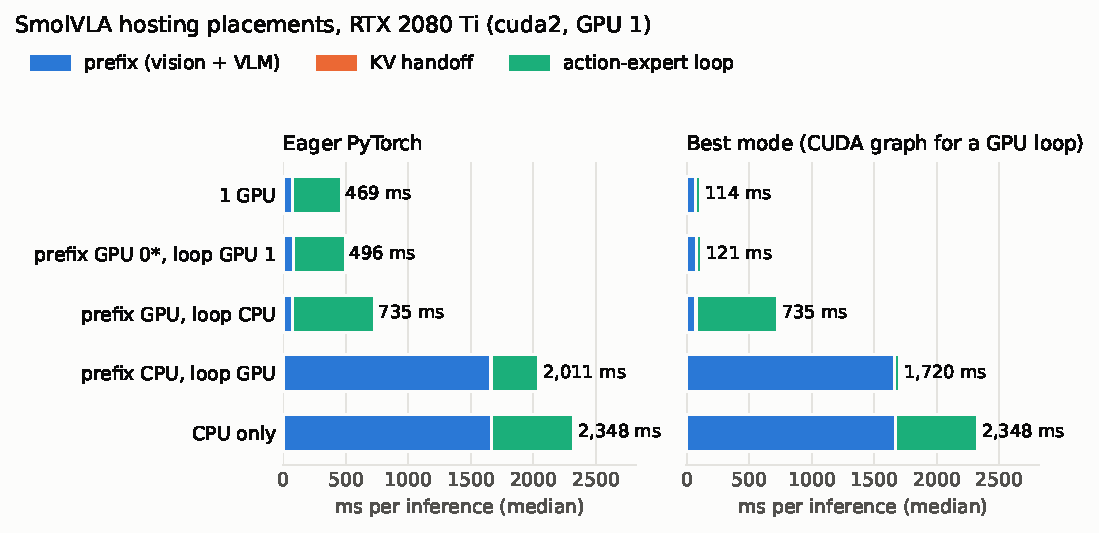
\includegraphics[width=\linewidth]{figures/placement_cuda2.pdf}
  \caption{SmolVLA step time per placement on cuda2, split into prefix, KV handoff (1.5 to
  3.2\,ms, too small to see) and action-expert loop. Left: eager PyTorch. Right: CUDA graph for
  the loop when it runs on a GPU. All rows use the healthy GPU~1, except the two-GPU row, whose
  prefix ran on GPU~0 while that GPU was stuck at a reduced clock (*, about 5\,ms slower).}
  \label{fig:placement}
\end{figure}

\paragraph{The handoff is cheap and the step is additive.} The KV cache is 4.9\,MB in 33
tensors. Moving it costs 1.5\,ms GPU to GPU, 2.8\,ms GPU to CPU and 3.2\,ms CPU to GPU (FP32
cache cast on the GPU), 1 to 3\% of the best single-GPU step (114\,ms). The parts timed alone
sum to the end-to-end step within 1.6\% in every placement, so a split placement can be
predicted from single-device runs:
$T(A,B) = T_\mathrm{prefix}(A) + n\,t_0 + S/\mathit{BW}_{A\to B} + T_\mathrm{loop}(B)$, with
$t_0$ and $\mathit{BW}$ from a copy calibration and each device's own baseline. The prediction
is within 0.1\% for the GPU-CPU split, 2.3\% (eager) and 0.6\% (graph loop) for the CPU-GPU
split, and 0.2\% (graph loop) and 2.5\% (eager) for the two-GPU split. Splitting does not
shorten one inference, since the halves run in sequence; it adds capacity, which hosting
several policies on one GPU (Section~\ref{sec:multipolicy}) provides more cheaply.

\paragraph{The CPU is not a useful host.} The prefix is 23 times slower on the CPU than on the
GPU, and CPU-only inference is 21 times slower than the best single-GPU step. The action loop
on 20 CPU threads takes 650\,ms, only 1.7 times the eager GPU loop (389\,ms): eager PyTorch is
so dispatch bound that a CPU comes close to it. With a CUDA graph the GPU loop takes 40\,ms, 16
times faster than the CPU. On the TITAN V host (24 threads) the CPU loop is 3.3 times the eager
loop and 14 times the graph loop.

\paragraph{Graph mode exposes a faulty GPU.} During these experiments GPU~0 of cuda2 ran the
graph loop in 54.1\,ms against 39.6\,ms on GPU~1, while the eager step was 482\,ms on both:
host-bound eager execution hides the difference and graph mode exposes it. GPU~0 is not slower
by design. A week earlier it held 1,950\,MHz under load and ran a C++ replay of the loop as
fast as GPU~1; since then it idles stuck in the P0 power state at 1,350\,MHz with no clock
event reason, and $1950/1350 = 1.44$ is close to the $1.37$ loop ratio. As with the TITAN V
(Section~\ref{sec:crossgpu}), the clock a GPU actually runs at sets the graph-mode latency.
Our runner now records every GPU's power state and clock and refuses a GPU that idles in P0.
% Needs \label{sec:crossgpu} on main.tex's "Cross-GPU accuracy" subsection (sustained-clock
% finding) and \label{sec:multipolicy} on the multi-policy subsection (branch
% shrikar/multipolicy-hosting); drop that clause if it is not in the paper.
